\documentclass[tikz,border=8pt]{standalone}
% Shared look for every TikZ diagram. Load with % Shared look for every TikZ diagram. Load with % Shared look for every TikZ diagram. Load with \input{../../tools/tikz-style.tex}
\usepackage[T1]{fontenc}
\usepackage{lmodern}
\renewcommand{\sfdefault}{lmr}  % diagrams use the same serif as the text
\usetikzlibrary{arrows.meta, positioning, shapes.geometric, calc, fit, backgrounds}
\definecolor{cblue}{HTML}{4C78A8}
\definecolor{corange}{HTML}{F58518}
\definecolor{cgreen}{HTML}{54A24B}
\definecolor{cred}{HTML}{E45756}
\definecolor{cpurple}{HTML}{B279A2}
\definecolor{cgrey}{HTML}{6B6B6B}
\tikzset{
  every picture/.style={font=\sffamily, line width=1.2pt},
  box/.style={draw=#1, fill=#1!12, rounded corners=4pt, align=center, inner sep=7pt, minimum height=1.1cm},
  box/.default=cgrey,
  arrow/.style={-{Stealth[length=3mm]}, draw=cgrey, line width=1.4pt},
  title/.style={font=\sffamily\bfseries\Large},
  note/.style={font=\sffamily\small, text=cgrey, align=center},
}
\AtBeginDocument{\hyphenpenalty=10000 \exhyphenpenalty=10000}

\usepackage[T1]{fontenc}
\usepackage{lmodern}
\renewcommand{\sfdefault}{lmr}  % diagrams use the same serif as the text
\usetikzlibrary{arrows.meta, positioning, shapes.geometric, calc, fit, backgrounds}
\definecolor{cblue}{HTML}{4C78A8}
\definecolor{corange}{HTML}{F58518}
\definecolor{cgreen}{HTML}{54A24B}
\definecolor{cred}{HTML}{E45756}
\definecolor{cpurple}{HTML}{B279A2}
\definecolor{cgrey}{HTML}{6B6B6B}
\tikzset{
  every picture/.style={font=\sffamily, line width=1.2pt},
  box/.style={draw=#1, fill=#1!12, rounded corners=4pt, align=center, inner sep=7pt, minimum height=1.1cm},
  box/.default=cgrey,
  arrow/.style={-{Stealth[length=3mm]}, draw=cgrey, line width=1.4pt},
  title/.style={font=\sffamily\bfseries\Large},
  note/.style={font=\sffamily\small, text=cgrey, align=center},
}
\AtBeginDocument{\hyphenpenalty=10000 \exhyphenpenalty=10000}

\usepackage[T1]{fontenc}
\usepackage{lmodern}
\renewcommand{\sfdefault}{lmr}  % diagrams use the same serif as the text
\usetikzlibrary{arrows.meta, positioning, shapes.geometric, calc, fit, backgrounds}
\definecolor{cblue}{HTML}{4C78A8}
\definecolor{corange}{HTML}{F58518}
\definecolor{cgreen}{HTML}{54A24B}
\definecolor{cred}{HTML}{E45756}
\definecolor{cpurple}{HTML}{B279A2}
\definecolor{cgrey}{HTML}{6B6B6B}
\tikzset{
  every picture/.style={font=\sffamily, line width=1.2pt},
  box/.style={draw=#1, fill=#1!12, rounded corners=4pt, align=center, inner sep=7pt, minimum height=1.1cm},
  box/.default=cgrey,
  arrow/.style={-{Stealth[length=3mm]}, draw=cgrey, line width=1.4pt},
  title/.style={font=\sffamily\bfseries\Large},
  note/.style={font=\sffamily\small, text=cgrey, align=center},
}
\AtBeginDocument{\hyphenpenalty=10000 \exhyphenpenalty=10000}

\newcommand{\hdr}[4]{\node[box=#4, minimum width=1.9cm, minimum height=0.8cm, inner sep=3pt, font=\sffamily\bfseries\small] at (#1,#2) {#3};}
\newcommand{\val}[4]{\node[draw=#4, fill=white, minimum width=1.9cm, minimum height=0.7cm] at (#1,#2) {#3};}
\begin{document}
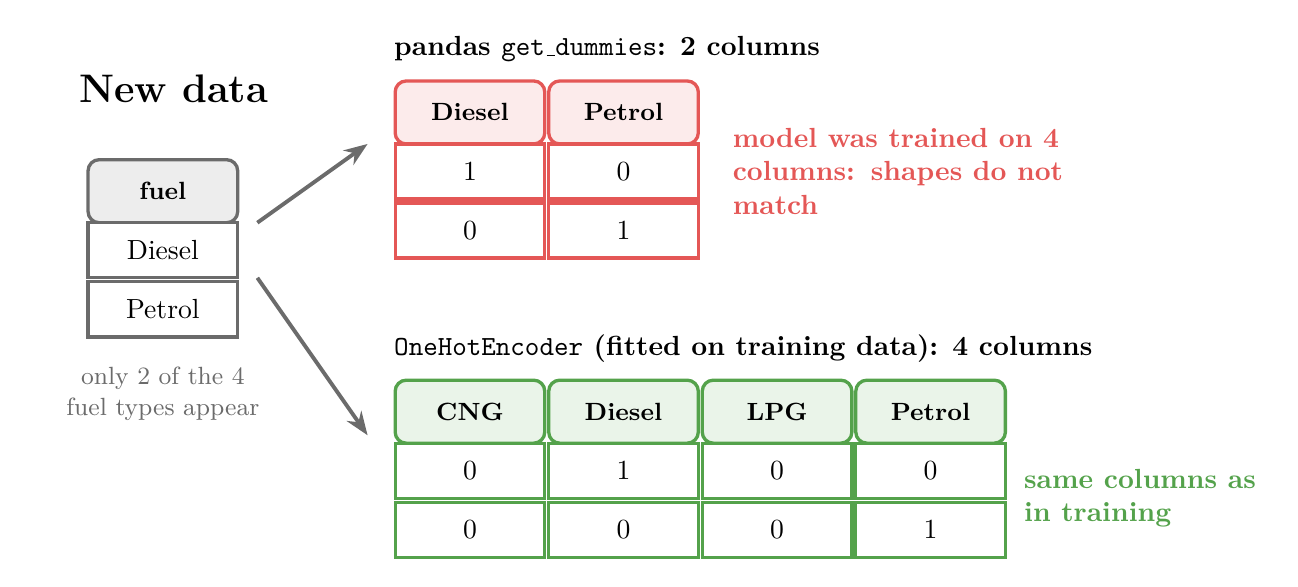
\begin{tikzpicture}
  % new data
  \node[title, anchor=west] at (-1.2,1.3) {New data};
  \hdr{0}{0}{fuel}{cgrey}
  \val{0}{-0.75}{Diesel}{cgrey}
  \val{0}{-1.5}{Petrol}{cgrey}
  \node[note, anchor=north, text width=3.2cm] at (0,-2.1) {only 2 of the 4\\ fuel types appear};
  \draw[arrow] (1.2,-0.4) -- (2.6,0.6);
  \draw[arrow] (1.2,-1.1) -- (2.6,-3.1);
  % get_dummies
  \node[font=\sffamily\bfseries, anchor=west] at (2.8,1.8) {pandas \texttt{get\_dummies}: 2 columns};
  \hdr{3.9}{1.0}{Diesel}{cred}
  \hdr{5.85}{1.0}{Petrol}{cred}
  \val{3.9}{0.25}{1}{cred}  \val{5.85}{0.25}{0}{cred}
  \val{3.9}{-0.5}{0}{cred}  \val{5.85}{-0.5}{1}{cred}
  \node[font=\sffamily\bfseries, text=cred, anchor=west, text width=4.4cm] at (7.1,0.25) {model was trained on 4 columns: shapes do not match};
  % OneHotEncoder
  \node[font=\sffamily\bfseries, anchor=west] at (2.8,-2.0) {\texttt{OneHotEncoder} (fitted on training data): 4 columns};
  \foreach \h [count=\j] in {CNG, Diesel, LPG, Petrol}
    \hdr{1.95+1.95*\j}{-2.8}{\h}{cgreen}
  \foreach \a/\b/\c/\d [count=\i] in {0/1/0/0, 0/0/0/1}
    \foreach \v [count=\j] in {\a,\b,\c,\d}
      \val{1.95+1.95*\j}{-2.8-0.75*\i}{\v}{cgreen};
  \node[font=\sffamily\bfseries, text=cgreen, anchor=west, text width=3.0cm] at (10.8,-3.9) {same columns as in training};
\end{tikzpicture}
\end{document}
